\section{Capacitive prototypes from related work}
% Table generated by Excel2LaTeX from sheet 'Tabelle1'
\begin{table}[htbp]	
	\centering
  \footnotesize
  \caption{Measuring layout and data processing of different prototypes from related works}
    \begin{tabularx}{\linewidth}{Xp{3.5cm}Xp{3.5cm}p{3.5cm}}
    \toprule
    \textbf{Name} & \textbf{Description} & \textbf{Application Areas} & \textbf{Measuring Layout} & \textbf{Data Processing} \\
    \midrule
    SensFloor \cite{lauterbach2009} & System for indoor localization and fall detection as floor underlay & Indoor Localization & Loading mode, variable number of sensors based on area size & Individual coding of zones on floor - analysis of activity based on trajectories \\
    TileTrack \cite{Valtonen2009a} & Indoor localization using transmitters below floor and receiver electrodes in wall or furniture & Indoor Localization & Transmit mode, large transmitter electrodes below floor, different receiving electrodes & Location by calculating center-of-gravity on most active tiles \\
    Touché \cite{Sato2012} & Swept-frequency sensing to detect different types of touches on a conductive material & Smart Appliances & Swept-frequency sensing, single electrode & SVM classification using features in different frequency ranges \\
    Botanicus Interactus \cite{poupyrev2012botanicus} & Using plant tissue as conductive material as application for swept-frequency sensing & Smart Appliances & Swept-frequency sensing, electrode coupled to plant tissue & SVM classification of touches that are transferred to input events \\
    Active capacitive sensing \cite{cheng2010active} & Conductive textile electrodes to sense different parameters of the human body, based on location & Physiological Sensing & Loading mode, single electrode attached to body part & Different filtering methods, based on electrode position, activity classification using LDA \\
    Spread spectrum sensor \cite{MacLachlan2004} & Single electrodes using a spread spectrum technique for improved sensitivity & Physiological Sensing & Loading mode, single electrode placed remotely & Spread spectrum technique to improve SNR, amplitude measurement for respiratory rate \\
    School of Fish \cite{smith1999thesis} & Array of shunt mode sensors that can track 3D position and orientation of two hands  & Gesture Interaction & Shunt mode, flexible array of sensors & Modeling hands as collection of spheres and fit into area based on sensor values and position \\
    Thracker \cite{Wimmer2006} & Four electrodes placed around display that can sense spatial position of hand in front of display and certain gestures & Gesture Interaction & Loading mode, four electrodes placed spatially around display & Position based on distance to electrodes or gesture based on nearest object to electrode \\
    GestIC \cite{microchip2013} & Shunt mode array enabling near distance gesture interaction above sensing area & Gesture Interaction & Shunt mode, four or five receiver electrodes & Positioning based on single proximity values and HMM-based gesture recognition \\
    \bottomrule
    \end{tabularx}%
  \label{tab:related_cap_proto}%
\end{table}%

While I already have presented capacitive systems in the related work section, they are briefly revisited here, to classify them given the specified application domains. Similar to the created prototypes I will give some additional detail regarding their measuring layout and data processing. The prototypes are shortly listed in Table \ref{tab:related_cap_proto}.

\subsection{Indoor localization}
One example system based on capacitive sensing is the previously presented TileTrack that uses a combination of transmit mode and center-of-gravity calculation between different floor tiles to calculate the position of multiple persons \cite{Valtonen2009a}. A second, already commercialized system is SensFloor that uses an integrated solution of capacitive sensors and wireless communication hidden below a floor covering that is able to detect the position of several users and other parameters such as falls, based on analyzing activity above single sensor areas or the movement trajectories over time \cite{lauterbach2009}.
\subsection{Smart Appliances}
Sato et al. have presented Touché, a swept-frequency capacitive sensor that allows distinguishing different types of touches on any suitable surface and medium \cite{Sato2012}. Some examples include recognizing different hand postures in liquids and touching different body parts to control mobile devices. Their system is based on analyzing a broader range of frequencies that have a different effect on the resulting capacitance. Using a classification method they are able to distinguish different categories of events. An-other example of this technology is touching different parts of a plant to control an interactive art installation  \cite{poupyrev2012botanicus}. Capacitive sensing provides the ability to add interactive features to many different appliances and allows for unobtrusive placement.
\subsection{Physiological sensing}
Capacitive proximity sensors can be used to measure various physiologi-cal parameters that are related to movement of dif-ferent body parts, including internal organs, most notably the heart. Cheng et al. have presented a system that allows measuring motions and shape changes of body parts using capacitive sensors em-bedded in garment \cite{cheng2010active}. They were able to detect swallowing and breathing rate. One example for an industrial application is non-contact electrocardiogram (ECG) sensing in cars, intended to detect drowsiness in drivers. MacLachlan presented a system that detects the respiratory rate of a person lying on a bed from a distance of up to 50cm using a single electrode and a highly sensitive sensing method based on spread spectrum methods that are commonly used in wire-less communication \cite{MacLachlan2004}.
Generally, capacitive proximity sensing is a powerful technology that is able to gather physio-logical information over a distance, while being unobtrusively integrated into various appliances. In applications that require this information, e.g. to detect the state of alertness or fitness of a user it is a viable alternative to body-worn sensors that are more intrusive by nature. \subsection{Gestural interaction}
Throughout the years there have been various at-tempts to enable the tracking of gestures in free air. Capacitive proximity sensors have been first presented almost 100 years ago by the Russian physicist Leon Theremin, who invented the eponymous touch-free electronic instrument [60] The theremin uses two electrodes to control pitch and volume of a generated sine wave. Capacitive hand tracking has been a research interest at MIT in the 1990s \cite{Smith1999a} and has been investigated recently by other groups, enabling touch control even through thick-er non-conductive materials [32], [61]. 
We introduced Thracker in section 2.6.2, that allows to either detect moving hand ges-tures or detect grasp actions in front of a screen  \cite{Wimmer2006}.

\begin{minipage}{\linewidth}
\centering
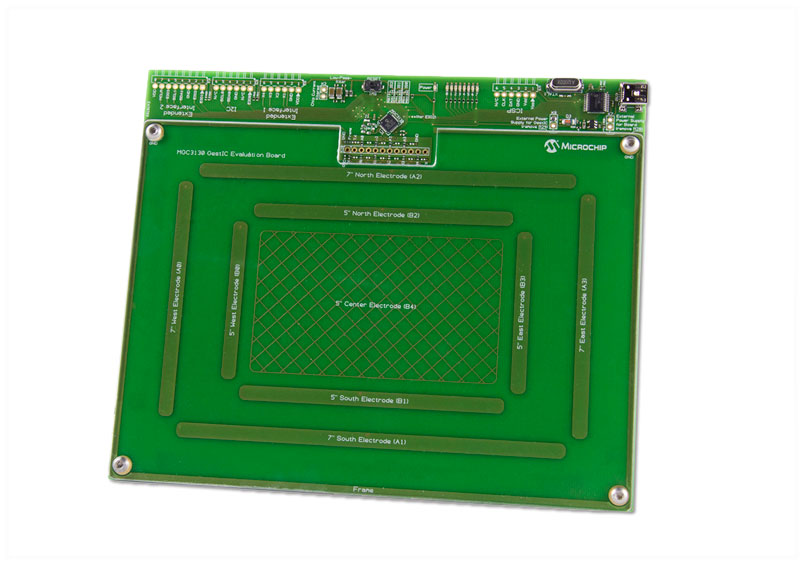
\includegraphics[width=0.5\textwidth]{images/gestic}
\captionof{figure}{GestIC® Sabrewing prototyping board \cite{microchip2013}}
\label{fig:prot_rel_gestic}
\end{minipage}

GestIC® by Microchip Technologies Inc. is a controller for electric near field 3D tracking based on capacitive proximity sensing \cite{microchip2013}. A prototyp-ing board is shown in Figure \ref{fig:prot_rel_gestic}. Using a set of several electrodes and on-board processing it is capable of tracking the 3D position of a hand and provides gesture recognition at a distance between 0 and 15 cm. 
